\documentclass[letterpaper,11pt]{article}
\pdfoutput=1

\usepackage[margin=2cm]{geometry}
\usepackage{graphicx}

\newcommand{\selected}{{\ensuremath s}}
\newcommand{\unselected}{{\ensuremath\slash\!\!\!\selected}}
\newcommand{\tot}{{\ensuremath\mathrm{tot}}}

\begin{document}

\begin{figure}
  \centering
  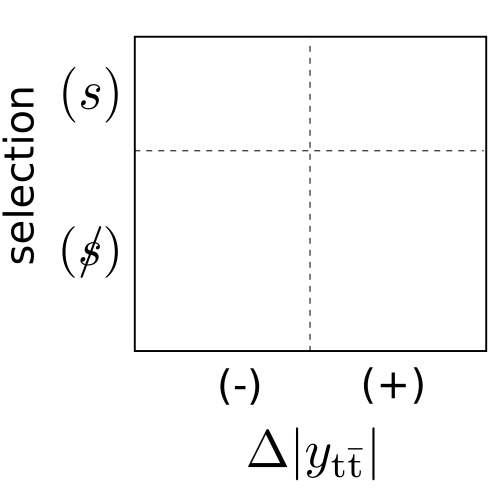
\includegraphics[width=0.3\linewidth]{axes}
  \caption{\label{axes} Four bins, selected ($\selected$) and unselected ($\unselected$) on
    the selection axis, and $(-)$ and $(+)$ on the axis of the the
    observable for which the asymmetry is of interest.}
\end{figure}

Consider a two dimensional distribution of four bins, where one axis
is a selection observable with bins (selected, $\selected$) and
(unselected, $\unselected$), and the other is an observable for which
the asymmetry is of interest, for example
$\Delta|y_{\mathrm{t\bar{t}}}|$, with bins $(+)$ and $(-)$.  Figure
\ref{axes} shows the axes. In a model $N$, the selection contains
$N_\selected=N_\selected^-+N_\selected^+$ events and has asymmetry
$\alpha_\selected$, while the unselected events number
$N_\unselected=N_\unselected^-+N_\unselected^+$ and may have a
different asymmetry $\alpha_\unselected$.  The counts in each bin are
given by
\[N_x^{\pm} = N_x(1\pm\alpha_x)/2,\qquad x\in\{\selected,\unselected\}\]
and the total asymmetry is given by
\[\alpha_\tot = \frac{N_\selected\alpha_\selected + N_\unselected\alpha_\unselected}{N_\selected+N_\unselected}.\]
Note that $\alpha_\selected\ne\alpha_\unselected$ if and only if the selection
efficiencies for the bins $(+)$ and $(-)$ are unequal.

\section{Two families of models}

Consider a two families of models of which $N$ is a member.  The
models $T(f)$ have an antisymmetric component proportional to that of
model $N$, with factor $f$,
\[T_x^{\pm}(f) = N_x(1\pm f\alpha_x)/2,\qquad x\in{\selected,\unselected,\tot}.\]
The asymmetries of a model $T(f)$ would be
\[\alpha_x^{(T)}=f\alpha_x, \qquad x\in\{\selected,\unselected,\tot\}.\]
The other family of models $U(w^\pm)$ is given by uniform reweighting
of the $(\pm)$ bins,
\[U_x^\pm(w^\pm) = N_x^\pm w^\pm(\mathrm{normalization\ constant}).\]
For simplicity of discussion, we will suppose $w^\pm=1\pm k$, but this
will not restrict the generality of our results.  Then
\[U_x^\pm(k) = \frac{N_x}{2}\left(\frac{1+k\alpha_x}{(1+k\alpha_\tot)}\pm\frac{\alpha_x+k}{1+k\alpha_\tot}\right), \qquad x\in\{\selected,\unselected,\tot\}.\]
The asymmetries of a model $U(k)$ would be
\[\alpha_x^{(U)} = \frac{\alpha_x+k}{1+k\alpha_x}, \qquad x\in\{\selected,\unselected,\tot\}.\]
In the general case $\alpha_\selected\ne\alpha_\unselected$, the
intersection of families $T(f)$ and $U(k)$ is $N=T(1)=U(0)$.  Some
notable features of each family of models include:
\begin{description}
\item[Models $T$]:
  \begin{itemize}
  \item Constant asymmetry proportions $\alpha^{(T)}:\alpha^{(T)}_\selected:\alpha^{(T)}_\unselected$
  \item Constant global selection ratio $T_\selected:T_\unselected$
  \item Variable bin selection ratios $T^\pm_\selected:T^\pm_\unselected$
  \end{itemize}
\item[Models $U$]:
  \begin{itemize}
  \item Constant bin selection ratios $U^\pm_\selected:U^\pm_\unselected$
  \item Variable global selection ratio $U_\selected:U_\unselected$
  \item Variable asymmetry proportions $\alpha^{(U)}:\alpha^{(U)}_\selected:\alpha^{(U)}_\unselected$
  \end{itemize}
\end{description}


\section{Extrapolation of total asymmetry from observations}

Suppose we wish to calculate the total asymmetry of a sample $D$ from
the observation of its selected components
$D_\selected^\pm=N_\selected(1\pm\alpha^{(D)}_\selected)/2$, based on
the model $N$.  We will generally find different results depending on
our hypothesis concerning which family of models, $T$ or $U$, better
describes $D$.  Supposing $D$ belongs to family $T$, we use the
property of constant ratio $\alpha_\tot/\alpha_\selected$ to
extrapolate the total asymmetry (template method), finding
\[[T]: \alpha_\tot^{(D)} = \left(\frac{\alpha_\tot}{\alpha_\selected}\right)\alpha^{(D)}_\selected.\]
Supposing $D$ belongs to family $U$ on the other hand, we use the
property of constant bin selection efficiencies to extrapolate total
asymmetry (unfolding method), finding
\[[U]: \alpha_\tot^{(D)} = \frac{\alpha^{(D)}_\selected(1-\alpha^2_\selected)N_\selected/N_\unselected + \alpha^{(D)}_\selected(1-\alpha_\selected\alpha_\unselected)+(\alpha_\unselected-\alpha_\selected)}{
                                                       (1-\alpha^2_\selected)N_\selected/N_\unselected + (1-\alpha_\selected\alpha_\unselected)+\alpha^{(D)}_\selected(\alpha_\unselected-\alpha_\selected)}{}.\]
%
Extrapolated total asymmetries using the template and unfolding
methods are shown as a function of selection asymmetry in the
observable $\Delta|y_{\mathrm{t\bar{t}}}|$ in Figure \ref{plot}, based
on a CMS lepton+jets selection ($\sim10\%$ efficient) of
$\mathrm{t\bar{t}}$ events generated by POWHEG, for which the total
asymmetry is $0.56\%$, and the selection asymmetry is $0.32\%$.
\begin{figure}
  \centering
  \includegraphics[width=0.7\textwidth]{plot}
  \caption{\label{plot} Extrapolation of the total asymmetry $A_c^y$
    as a function of the asymmetry of the observable
    $\Delta|y_{\mathrm{t\bar{t}}}|$ in a CMS lepton+4jets selection
    ($\sim$10\% efficient), using two different 2-bin methods based on
    {\sc POWHEG} $\mathrm{t\bar{t}}$ simulation, and asumming perfect
    resolution.  The bisector shows what the extrapolation would be if
    the asymmetry were expected to be selection independent.  Both
    extrapolation methods reduce to the bisector in the case that
    $\alpha_\selected=\alpha_\unselected=\alpha_\tot$, which is not
    the case for POWHEG.}
\end{figure}
These three numbers (total asymmetry, selection asymmetry, selection
efficiency) from any simulation are sufficient to generate the
extrapolation curves for 2-bin versions of both the template method
and the unfolding method.  Clearly the two methods coincide in their
extrapolations only for an observed selection asymmetry equal to that
modeled by the simulation, and diverge quite rapidly from that
intersection.

%\subsection{Template Strategy}
%Following the template strategy we have so far employed, the weights
%which symmetrize and antisymmetrize the original distribution after
%integrating over the selection axis would be
%\[W^\pm_{\mathrm{symm}} = (1\pm\alpha)^{-1},\]
%\[W^\pm_{\mathrm{anti}} = \pm\alpha(1\pm\alpha)^{-1}.\]
%The templates for the selection would be
%\[T^{\pm}_{\mathrm{symm}} = \frac{N_\selected}{2}\frac{1\pm\alpha_\selected}{1\pm\alpha},\]
%\[T^{\pm}_{\mathrm{anti}} = \pm\alpha\frac{N_\selected}{2}\frac{1\pm\alpha_\selected}{1\pm\alpha},\]
%and the parametrized template model would be
%\[T^{\pm}(f) = T^{\pm}_{\mathrm{symm}} + f\cdot T^\pm_{\mathrm{anti}} = \frac{N_\selected}{2}\frac{1\pm\alpha_\selected}{1\pm\alpha}(1\pm f\cdot\alpha).\]
%Our expectation has been that $T^\pm(f) = T^\pm_\selected$ when $f=F$, but
%that is clearly only the case if $F=f=1$ or $\alpha=\alpha_\selected$.  The
%former condition is useless for a measurement, while the latter
%condition is generally unmet, and is particularly untrue in the cases
%of our subselections at extremes of $\mathrm{t\bar{t}}$ system
%rapidity and mass.
%

\section{Argument for Template Method}

It is clear from simulation that asymmetry is shaped by the selection.
A key question is whether this shaping is induced by asymmetric
selection criteria, or rather due to modeled differential asymmetry
between unselected and selected events.  If the former, constant bin
selection efficiencies would be expected, and the unfolding method is
appropriately used to extrapolate total asymmetry from observations,
while application of the template method would be incorrect.  In the
latter case however, extrapolations from the unfolding method would be
misleading, while extrapolating with the template method would be
defensible.  The possibility that asymmetry could be shaped by both
the former and the latter is admitted.

A test for asymmetric selection criteria would necessarily control for
all modeled differential asymmetry, the easiest method of which would
be to check the asymmetry of a selection from a sample with no
assymetry at all. It would not be sufficient to reweight events as a
function of only the asymmetry observable to acheive symmetry in just
that dimension, for example, since the selection presumably cuts
through many other dimensions which would still retain a non-zero
differential asymmetry after reweighting.  Selection criteria that
could induce asymmetry can be imagined if, for example, lepton
reconstruction efficiencies were charge-dependent.

We note that differential $\mathrm{t\bar{t}}$ charge asymmetry is
expected along many kinematic dimensions, including system mass,
system transverse momentum, system rapidity, and number of extra jets,
none of which are expected to be uniform in selection efficiency.

\section{Reconstruction effects}

Suppose our 

\end{document}
